\documentclass{article}

\newcommand{\HorRule}{\color{Black}\rule{14cm}{1pt}} % Defines the gold horizontal rule around the title

\setlength{\columnsep}{1cm}
\usepackage[utf8]{inputenc}
\usepackage{geometry}
\geometry{
 a4paper,
 left=30mm,
 right=30mm,
 top=30mm,
 bottom=30mm,
 }
\pagenumbering{arabic}
\usepackage[dvipsnames]{xcolor}
\usepackage{amsmath}
\usepackage{amsthm}
\usepackage{amssymb}
\usepackage{graphicx}
\usepackage{url}
\usepackage[titletoc,title]{appendix}
\linespread{1.3}
\usepackage{multicol}
\usepackage[margin=10pt,font={sf,normalsize,stretch=0.8},labelfont=bf,
labelsep=period]{caption}

 
\newtheorem{definition}{Definition}[section]
\newtheorem{result}[definition]{Result}
\newtheorem{theorem}{Theorem}[section]
\newtheorem{corollary}{Corollary}[theorem]
\newtheorem{lemma}[theorem]{Lemma}
 
\usepackage{tabularx,booktabs}
\newcolumntype{Y}{>{\centering\arraybackslash}X}
 
% Document starts here
% --------------------
\begin{document}

% Title page

\begin{titlepage}
   \begin{center}
        \vspace*{2cm}
        \LARGE
        \textbf{COMP0047 Data Science}

        \Large
       % \vspace{0.75cm}
        Coursework
    
        \HorRule\vspace{3.5cm}
        {\fontfamily{phv}\selectfont
        \textbf{The Suburbia Effect: \\}
        \vspace{0.25cm}
        \textbf{Do restaurants in the suburbs achieve systematically higher ratings than those in the city?}}

        \large
        \vspace{4cm}
        \HorRule
        \vspace{1cm}
        \textit{Date:\\} \textbf{April 2022} \\
        \vspace{0.45cm}
        \textit{Word Count:\\} \textbf{1495} \\ \text{(\LaTeX)}
            
   \end{center}
\end{titlepage}


\section{Introduction}
There are a number of stereotypes associated with the city and the suburbs. The city is thought of as a bustling, noisy environment in which people are under constant stress. Whilst the suburbs evoke images of carefully manicured lawns, open spaces, and happy family life \cite{adams1992happiness}. \par

But do these stereotypes apply to all aspects of life? In particular, are people in the suburbs more positive when it comes to reviews? We sought to answer this question for one specific category of businesses – restaurants – and proposed the following hypothesis: Restaurants in the suburbs achieve systematically higher ratings than those in the city. 


\section{Data \& Methodology}
\subsection{Data Pre-processing}
We have used two subsets of the most recent Yelp dataset \cite{yelp_academic_dataset}, `Reviews' and `Business'. On the Yelp website, business ratings are rounded to the nearest half star \cite{luca2016reviews}. If we were to simply use these figures we would have been presented with a discrete (and somewhat restricted) view which, for our purposes, was unsuitable as many of the intended statistical tests required a continuous distribution. \par

To address this issue, we took an average of the stars given in the `Review' dataset. Of course, this is the true star rating sitting behind the rounded rating in the `Business' dataset. As our hypothesis is purely focused on numerical ratings, we chose to drop all other fields, leaving only \textit{business\_id} and \textit{stars}. We then left-joined the reduced `Review' dataset onto the `Business' dataset to produce an accurate picture of the star ratings for each business. In addition, our hypothesis only considered restaurants, hence, we dropped all entries for which the field \textit{attributes} did not contain restaurants. \par

\begin{figure*}[ht]
    \centering
    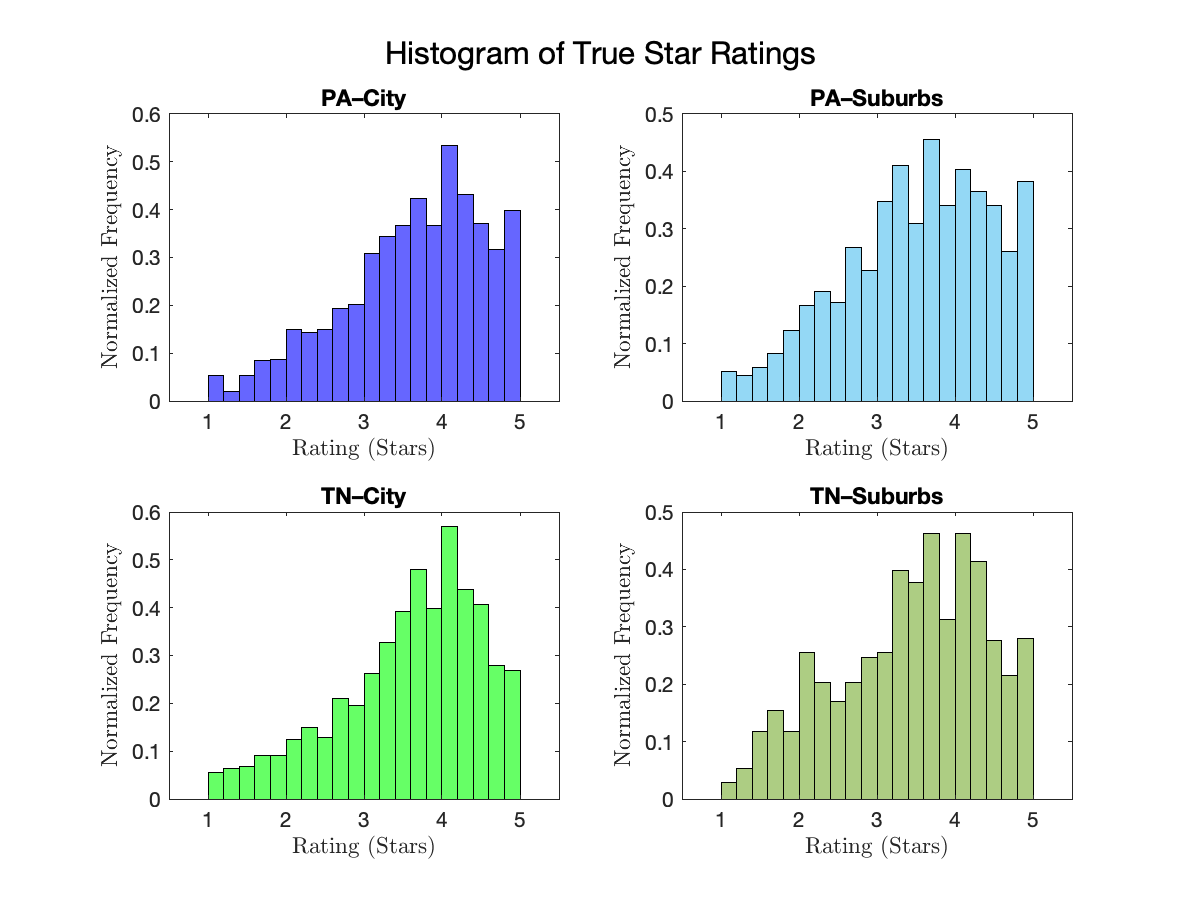
\includegraphics[trim={0 0 0 1cm},clip,width=\textwidth]{Histogram.eps}
    \caption{The histograms show the distribution of true star ratings for restaurants in each of the four defined areas. We grouped the data into 20 bins, each of width 0.2 stars, to provide a more detailed view of the distribution. We can clearly see each distribution is negatively skewed, which provides strong evidence that they are not normally distributed.}
    \label{fig:1}
\end{figure*}

\subsection{City vs. Suburbs}
To increase the robustness of our results, and to broaden our analysis, we chose to consider two metropolitan areas. Unfortunately, the most recent Yelp dataset has a North American focus and as such we were restricted to cities in the U.S. or Canada. We chose to analyse the Philadelphia (PA) and Nashville (TN) metropolitan areas for the following reasons. \par

Firstly, we wanted the geographical layout of the two areas to be sufficiently different so as not to introduce any subtle landscape bias\footnote{We introduce a new term, \textit{Landscape Bias}, to refer to areas possessing similar geographical properties, e.g. two desert based cities.} which may overstate our results. Philadelphia, located at the intersection of three northern states, and Nashville, rather isolated in the centre of Tennessee satisfied this requirement. \par

Secondly, we required each metropolitan area to contain a sufficiently large amount of restaurants to produce a reliable distribution of star ratings. The Philadelphia metropolitan area contained a total of 11,500 restaurants, and the Nashville metropolitan area contained 4,400. It is worth noting that as we are not comparing the areas with one another, we are simply analysing each internally, their unbalanced nature is not of concern. \par

Finally, we needed the ability to separate the `city' and the `suburbs'. Naturally, this is rather subjective, so we relied on the invaluable \textit{city} field in the dataset for our definition.

\begin{definition} 
If the location listed in the city field of the dataset matches the name of the metropolitan area, we classify the restaurant as the \textbf{city}. Otherwise, we classify the restaurant as the \textbf{suburbs}.
\end{definition}

Consequently, we were able to separate our dataset into four discrete sub-datasets. These were: \textit{PA–City} (5,500); \textit{PA–Suburbs} (6,000); \textit{TN–City} (2,400); and \textit{TN–Suburbs} (2,000). The number in brackets indicates the size of each sub-dataset. For our purposes, we considered the pairs to be sufficiently balanced and thus concluded our pre-processing. \par

\subsection{Methodology}
We turn our attention to the methods used to test our hypothesis. This required an iterative approach, addressing smaller components in stages. 

\subsubsection*{Shapiro–Wilks Normality Test}
Our first, and perhaps most fundamental, step was to test the null hypothesis that the true star ratings for our four sub-datasets were normally distributed. The histograms (Figure 1) provided visual indication that this was false, however, to provide statistical confirmation we performed the Shapiro–Wilks test for normality. We chose to use the Shapiro–Wilks method over alternatives such as the Anderson-Darling test as it offered superior performance when testing against normal distributions with non-specified mean and variance \cite{razali2011power}. 

\subsubsection*{Kolmogorov–Smirnov Test}
Next, we focused on the two sub-datasets for each metropolitan area. For our overarching hypothesis to have statistical basis, we required the distribution of true star ratings for the city and the suburbs to be different.\par

\begin{equation}
    D_{city;suburbs} = \sup_{x} | F_{1,city}(x) - F_{2,suburbs}(x) |
\end{equation}

We computed the test statistic (1) for the null hypothesis that our true star rating distributions for the two sub-datasets of each metropolitan area were identical. Whilst this test is rather sensitive, we believed the sample size of each sub-dataset was sufficient to be considered a reliable indicator.

\subsubsection*{Mann–Whitney U Test}
We then proposed testing the null hypothesis that the means of the city sub-datasets were less than the means of the suburbs sub-datasets. We used the one-sided Mann–Whitney U test. This was deemed the most appropriate because: \textit{(i)} we have used the true star ratings which we considered a continuous distribution; \textit{(ii)} we had confidence ratings in the city and suburbs were independent; and \textit{(iii)} star ratings are ordinal (i.e. they can be ranked). This meant our sub-datasets satisfied the underlying assumptions of the test. \par

Technically, the Mann–Whitney U test is not a true test for the difference in means \cite{macfarland2016mann}. We can merely interpret it as testing whether the difference in central tendency between two populations is different than zero. For our purposes though, we used this as a proxy to indicate whether the city and suburbs have statistically significant different means.

\subsubsection*{Kernel Density Estimation}
We also wanted to produce a non-parametric probability density function using a Gaussian kernel (2). This served the dual purpose of highlighting and providing visual confirmation of the differences between distributions, and could form the basis of future work. 

\begin{equation}
    \mathbb{P}(x;h;\{x_i\}_{i \in T}) = \frac{1}{N_{T} \sqrt{2 \pi h^2}} \sum_{i\in T} exp\left(-\frac{1}{2} \left(\frac{x - x_i}{h}\right)^2\right)
\end{equation}

To compute the kernel density, we required an appropriate bandwidth parameter $h$. Traditionally, maximum log-likelihood (3-4) is used to compute $h_{opt}$, that is:

\begin{equation}
    h_{opt} = \arg\max_{h} \log \mathcal{L}(h).
\end{equation}
Where,
\begin{equation}
    \log \mathcal{L}(h) = \sum_{j \in V} \log \mathbb{P}(x_{j};h;\{x_i\}_{i \in T}).
\end{equation}
However, during our analysis the computed value of $h_{opt}$ (3) was unusually small, $O(10^{-3})$, which gave an uneven and inappropriate Kernel PDF, despite the use of both training and validation sets. Instead, we found success using the `rule of thumb' \cite{silverman2018density} bandwidth parameter, $h_{est}$, given by,
\begin{equation}
    h_{est} = \left( \frac{4 \hat{\sigma}}{3 N_{T}} \right)^{\frac{1}{5}}.
\end{equation}

Where $\hat{\sigma}$ is the standard deviation of the training set.

\section{Results}
We now present the results of the analysis. 

\begin{table*}[ht]
\begin{center}
%\footnotesize
\begin{tabularx}{\textwidth}{c *{5}{Y}}
\toprule
\multicolumn{6}{c}{\textbf{Statistical Test Results}} \\
\toprule
 &  
 & \multicolumn{1}{c}{Kolmogorov–}
 & 
 & \multicolumn{1}{c}{Mean Star} 
 & 
 \\
 Sub-dataset
 & \multicolumn{1}{c}{Shapiro–Wilks} 
 & \multicolumn{1}{c}{Smirnov} 
 & \multicolumn{1}{c}{Mann–Whitney U} 
 & \multicolumn{1}{c}{Rating}
 & \multicolumn{1}{c}{Bandwidth}
 \\
 & \multicolumn{1}{c}{$p$-value} 
 & \multicolumn{1}{c}{$p$-value} 
 & \multicolumn{1}{c}{$p$-value} 
 & \multicolumn{1}{c}{$\hat{\mu}$}
 & \multicolumn{1}{c}{$h_{est}$}
 \\
\midrule
\multicolumn{1}{l}{PA–\textit{City}} 
 & \multicolumn{1}{c}{$6\times10^{-37}$} 
 & \multicolumn{1}{c}{$1\times10^{-10}$}
 & \multicolumn{1}{c}{$1\times10^{-9}$} 
 & $3.61$ 
 & $0.22$
 \\
 \multicolumn{1}{l}{PA-\textit{Suburbs}} 
 & \multicolumn{1}{c}{$4\times10^{-35}$} 
 & \multicolumn{1}{c}{–} 
 & \multicolumn{1}{c}{–} 
 & $3.52$ 
 & $0.21$
 \\
 \multicolumn{1}{l}{TN–\textit{City}} 
 & \multicolumn{1}{c}{$6\times10^{-28}$} 
 & \multicolumn{1}{c}{$2\times10^{-10}$} 
 & \multicolumn{1}{c}{$3\times10^{-11}$} 
 & $3.59$ 
 & $0.25$
 \\
 \multicolumn{1}{l}{TN–\textit{Suburbs}} 
 & \multicolumn{1}{c}{$1\times10^{-19}$} 
 & \multicolumn{1}{c}{–} 
 & \multicolumn{1}{c}{–} 
 & $3.41$ 
 & $0.29$
 \\
\bottomrule
\end{tabularx}
\end{center}
\caption{The table summarises our results of the statistical tests performed on each of the four defined areas. The Kolmogorov–Smirnov and Mann–Whitney U tests are only displayed for the city as the tests required both the city and the suburbs as inputs, hence, only produced one test statistic. All of our results can be classed as significant. It is worth noting though, that more extreme $p$-values are not proof that the alternative hypothesis is true, but merely indicate a greater level of confidence that the null hypothesis is false. We have also provided the mean star rating, $\hat{\mu}$, and estimated bandwidth parameter, $h_{est}$, for each area. We can see that for both PA and TN, the city has a higher average rating than the suburbs. }
\end{table*}

We can see from the results in Table 1, our $p$-values were sufficiently small that we could reject each null hypothesis at the 5\%, 1\%, and 0.1\% significance levels. The histograms (Figure 1) gave us confidence that our Shapiro–Wilks test would indicate non-normality, meaning that our subsequent use of non-parametric tests was appropriate. The Kolmogorov–Smirnov test results indicate that the distributions are indeed different, which we can visually confirm using our kernel density estimation (Figure 2). Likewise, the Mann–Whitney U test results show that the means are sufficiently different. In addition, we present the computed true star rating sample mean and bandwidth parameters (5) for comparison. Note that for both the Kolmogorov–Smirnov and Mann–Whitney U tests, we only present the $p$-value for the \textit{City} sub-datasets. This is because we tested the two sub-datasets against one another, not individually.

\begin{figure*}[t]
    \centering
    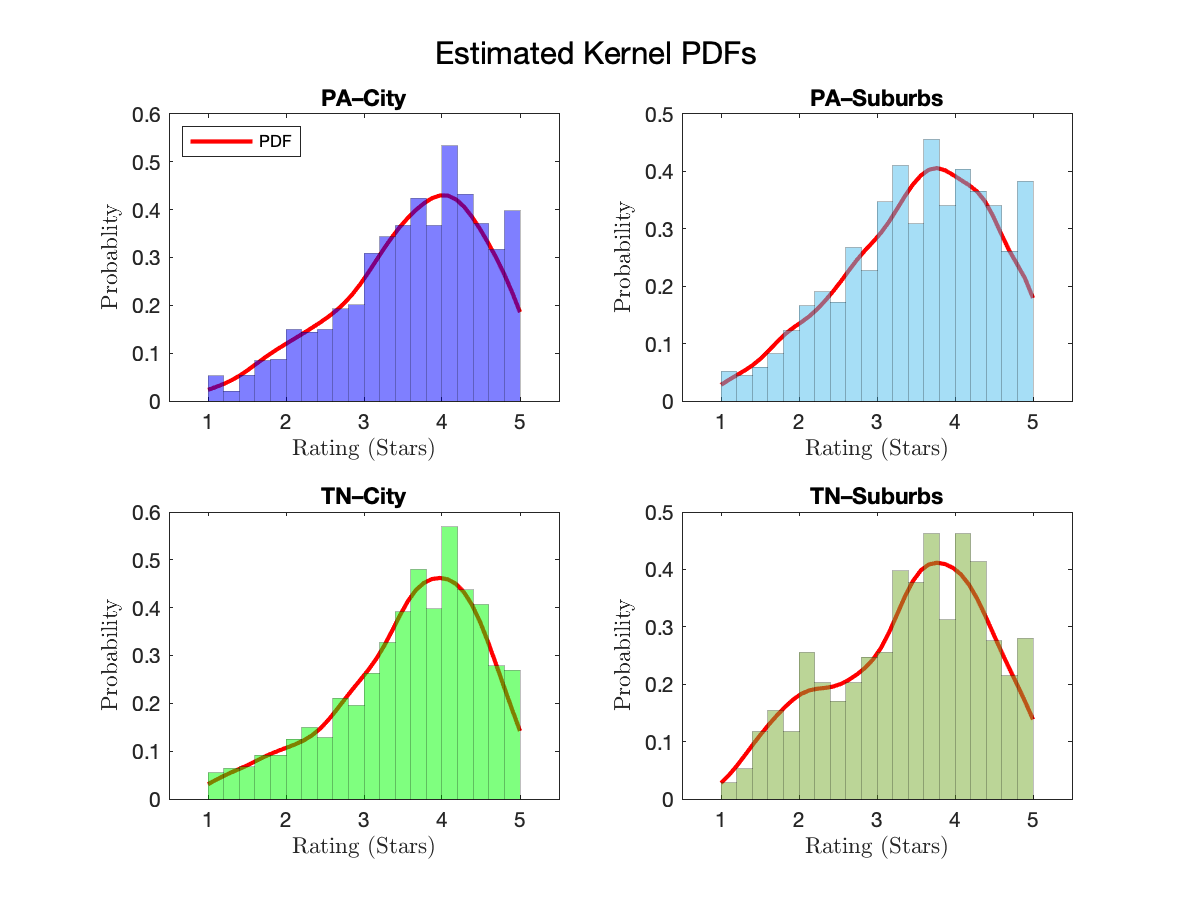
\includegraphics[trim={0 0 0 1cm},clip,width=\textwidth]{kerneldensity.eps}
    \caption{We have plotted the estimated probability density functions in red, found using a Gaussian Kernel (2), over our empirical histogram distributions. Our bandwidth parameters (top-left, clockwise) were: 0.22, 0.21, 0.29, and 0.25. This provides further visual confirmation that our initial hypothesis: Ratings in the city are systematically higher than those in the suburbs, is false. This can be seen by the 'fat' left tail of both suburbs distributions, with TN being more prominent. These kernel PDFs could be used in future research.}
    \label{fig:2}
\end{figure*}

\section{Discussion}
Returning to our research question, it seems our original hypothesis was incorrect. We can, in fact, infer the exact opposite: that restaurant ratings in the \textit{city} attract systematically higher ratings on a statistical basis than those in the suburbs. \par

This is an interesting outcome, although caution is advised. Whilst statistically significant, our results have little bearing in the real world. As mentioned in Section 2.1., Yelp rounds ratings to the nearest half star. This means that all mean ratings listed in Table 1 would be rounded to 3.5 stars, thus it is only for the true underlying continuous ratings that we can infer this outcome. \par

However, this does not prevent us from suggesting that our results seem  intuitive for several reasons. Firstly, from an economic perspective, restaurants in the city are more likely to offer higher salaries to staff. This means that both waiting staff and chefs are more likely to seek out work in the city, leading to increased competition and thereby theoretically increasing the quality of the restaurant, which would naturally lead to higher ratings from customers. \par

Secondly, it could be that restaurants in the city receive greater influence from other sources, perhaps from another state or country, which could boost innovation and introduce new cuisines that weren't available previously. Assuming the restaurant provided goods and services of sufficient quality, the uniqueness of the offer could lead to higher ratings. \par

Finally, one can naturally assume that competition in the city is fierce. The paradigm `survive or die' is likely to hold and we can infer that ratings in the city are, in general, higher because the restaurant is unlikely to survive otherwise. This point leads to an interesting question and possible extension of this work. Does our analysis suffer from survivorship bias? One approach could be to widen the time-window of the Yelp data and include those restaurants that shut down during that period. An alternative proposal, could be to repeat the analysis for different metropolitan areas – particularly those outside of North America – and understand whether our results appear consistently. \par


\bibliographystyle{IEEEtran}
\bibliography{bibliography} % Entries are in the bibliography.bib file

\end{document}
